\section{Polyfills}\label{polyfills-mit-webcomponents.js}

In den Abschnitten \ref{custom-elements} bis \ref{html-imports} wurde gezeigt, wie die Web-Components-Technologien funktionieren und ob diese bereits in allen Browsern unterstützt werden. In diesem Abschnitt wird genauer darauf eingegangen was Polyfills sind. Ebenso wird auf deren Performance eingegangen und wie sie die Browserunterstützung der Web-Components-Technologien verbessern.


\subsection{Native Browserunterstützung von Web Components}\label{native-browserunterstuxfctzung-von-web-components}

In den einzelnen Unterkapiteln zu den Technologien wurde jeweils kurz gezeigt, ob diese von den Browsern unterstützt wird oder nicht. Es wurde deutlich, dass Chrome und Opera bisher die einzigen Vorreiter sind. Bis auf \ac{HTML} Templates, welche von allen modernen Browsern unterstützt werden, unterstützen sie als einzige alle Technologien. \cite{citeulike:13914379}

\begin{description}
  \item[Chrome] Hat alle Spezifikationen der Web-Component-Standards ab Version 43 komplett implementiert.
  \item[Firefox] Unterstützt nativ \ac{HTML} Templates. Custom Elements und Shadow \ac{DOM} sind zwar implementiert, müssen aber über das Flag \texttt{dom.webcomponents.enabled} manuell in den Entwicklereinstellungen aktiviert werden. \ac{HTML} Imports werden, wie in Kapitel \ref{html-imports} erwähnt, bis auf Weiteres nicht unterstützt.
  \item[Safari] \ac{HTML} Templates werden ab Version 8 unterstützt, Custom Elements und Shadow \ac{DOM} befinden sich in der Entwicklung (Stand Januar 2016), \ac{HTML} Imports werden jedoch nicht unterstützt.
  \item[Internet Explorer] Als einziger Browser unterstützt der Internet Explorer keine der Web-Components-Technologien. Die Unterstützung wird -- auf Grund der Einstellung der Entwicklung und des Wechsels zu Microsoft Edge -- auch nicht nachträglich implementiert werden.
  \item[Microsoft Edge] Templates werden ab Version 13 unterstützt, über die Entwicklung der restlichen Technologien kann allerdings abgestimmt werden \cite{citeulike:13914237}.
  \item[Mobile Browser] Alle Technologien werden bisher nur auf Android in den Browsern Chrome für Android, Opera und Android Browser unterstützt.
\end{description}

Die Browserunterstützung der Technologien der Web Components ist momentan also noch verhalten. Das bedeutet jedoch nicht, dass sie noch nicht verwendet werden können. Mittels JavaScript besteht die Möglichkeit, die Technologien den Browsern beizubringen, welche sie nicht unterstützen. Ein solches JavaScript wird ``Polyfill'' genannt.


\subsection{Polyfill webcomponents.js}\label{polyfill-webcomponents.js}

\begin{quote}
A polyfill, or polyfiller, is a piece of code (or plugin) that provides the technology that you, the developer, expect the browser to provide natively. \cite{citeulike:13914241}
\end{quote}

Mit Hilfe von Polyfills können die Technologie-Lücken der Browser also auf mehrere, unterschiedliche Arten (``Poly'') gefüllt (``fill'') werden \cite{citeulike:13914234}. Eine Sammlung an Polyfills Technologien der Web Components bildet das JavaScript webcomponents.js. Es wurde von Google im Rahmen von Polymer entwickelt und hat eine dermaßen weite Verbreitung erfahren, dass es auszugliedern wurde. Somit kann es auch unabhängig von der Benutzung von Polymer eingesetzt werden \cite{citeulike:13914239}.


\subsection{Browserunterstützung}\label{polyfills-browserunterstuetzung}

Mit dem Einsatz der webcomponents.js Polyfills werden die Web Components auch auf den Internet Explorer, Firefox sowie Safari portiert. Eine detaillierte Matrix der Browserunterstützung der Web Components mit Einsatz der Polyfills ist in Abbildung \ref{fig:bdwctmwcjs} \cite{citeulike:13914238} dargestellt.

\begin{figure}[htbp]
 \centering
 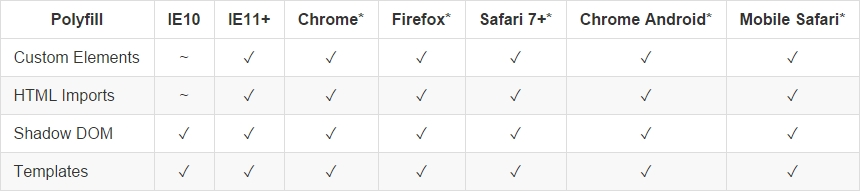
\includegraphics[width=\linewidth]{kapitel2/bilder/6-webcomponentsjs-browserunterstuetzung}
 \caption{Browserunterstützung der Web Components Technologien mit webcomponents.js}
 \label{fig:bdwctmwcjs}
\end{figure}

Jedoch werden die Technologien der Web Components auch mit Einsatzes der Polyfills nur von den aktuelleren Versionen des jeweiligen Browsers unterstützt. Darunter fallen jedoch weiterhin nicht ältere Browser, wie beispielsweise der Internet Explorer in Version 8 und 9. Des Weiteren werden einige Technologien auf Grund der Komplexität nicht komplett simuliert. Hier muss bei einigen Technologien auf folgende Punkte geachtet werden.

\begin{description}
  \item[Custom Elements] Die \ac{CSS}-Pseudoklasse \texttt{:unresolved} wird nicht unterstützt.
  \item[Shadow \ac{DOM}] Das Shadow \ac{DOM} kann auf Grund der Kapselung nicht komplett künstlich simuliert werden, dennoch versucht das webcomponents.js Polyfill einige der Features zu simulieren. So sprechen definierte \ac{CSS}-Regeln alle Elemente in einem künstlichen Shadow Root an -- als würde man den \texttt{\textgreater{}\textgreater{}\textgreater{}} Selektor benutzen -- auch die \texttt{::shadow} und \texttt{::content} Pseudoelemente verhalten sich so.
  \item[\ac{HTML} Templates] Templates, welche mit einem Polyfill erzeugt werden, sind nicht unsichtbar für den Browser, ihre enthaltenen Ressourcen werden also schon beim initialen Laden der Seite heruntergeladen.
  \item[\ac{HTML} Imports] Die zu importierenden \ac{HTML}-Dateien werden mit einem \ac{XHR}, und somit asynchron heruntergeladen, selbst wenn das \texttt{async}-Attribut (siehe Abschnitt \ref{asynchrones-laden-von-imports}) nicht gesetzt ist.
\end{description}


\subsection{Performance}\label{performance}

Das webcomponents.js-JavaScript \cite{citeulike:13914238} bringt mit seiner Größe von 116 KB einen großen Umfang mit, was sich negativ auf die Ladezeiten der Webseite auswirkt. Des Weiteren müssen die von den Browsern nicht unterstützten und ignorierten \ac{CSS}-Regeln -- wie \texttt{::shadow} oder \texttt{::slotted} -- mit Regular Expressions nachgebaut werden, was momentan 40 Stück sind. Das macht die Polyfills extrem komplex und träge. Die Funktionen zum Traversieren des \ac{DOM}s müssen angepasst werden, damit nur die richtigen Elemente angezeigt werden und eine Shadow Boundary simuliert wird. Diese werden mit 42 Wrappern umgesetzt, was wie die Regular Expressions zur Simulation der \ac{CSS}-Regeln sehr aufwändig ist. Allerdings können einige Funktionen wie \texttt{window.document} schlichtweg nicht überschrieben werden. Im Allgemeinen wird die \ac{DOM}-\ac{API} stark verlangsamt, wodurch die Performance -- speziell auf mobilen Geräten -- drastisch sinkt und mitunter nicht tolerierbar ist \cite{citeulike:13886251}.


\subsection{\texorpdfstring{Request-Minimierung mit ``Vulcanize''}{Request-Minimierung mit Vulcanize}}\label{request-minimierung-mit-vulcanize}

Webseiten können viele verschiedene, modular aufgebaute JavaScript-Dateien, Stylesheets, etc. beinhalten, welche die Anzahl an Requests erhöhen. Um die Anzahl an Requests zu verringern gibt es in der Webentwicklung bereits mehrere verschiedene Hilfsmittel. So werden die einzelnen Stylesheets oder auch JavaScript Dateien zu einer einzigen Datei konkateniert, sodass für das komplette Styling und JavaScript jeweils eine große Datei entsteht, welche nur einen Request an den Server benötigen. Zusätzlich kann sie anschließend noch minifiziert werden, um ihre Größe zu verringern und die Ladezeiten zu verkürzen. Selbiges Prinzip kann auch auf die \ac{HTML} Imports angewendet werden. Google stellt hierfür das Tool Vulcanize \cite{citeulike:13879681} bereit, welches serverseitig ermöglicht, einzelne kleine Web Components in einer einzigen, großen Web Component zusammenzufassen. Benannt nach der Vulkanisation, werden metaphorisch die einzelnen Elemente in ein beständigere Materialien umgewandelt. Vulcanize reduziert dabei eine \ac{HTML}-Datei und ihre zu importierenden \ac{HTML}-Dateien in eine einzige Datei. Somit werden die unterschiedlichen Requests in nur einem einzigen gebündelt und die Ladezeiten sowie die benötigte Bandbreite minimiert.

